\documentclass[11pt]{article}

\usepackage[margin=1in]{geometry}
\usepackage{booktabs}
\usepackage{graphicx}
\usepackage{hyperref}
\usepackage{longtable}

\title{Celestial Boundary Toy Probes and Claim-Gated Physics Bridge: Phase 63.1 Release for HAOS-IIP}
\author{Tomislav Rupi\'c \\ Independent Researcher}
\date{April 2026}

\begin{document}

\maketitle

\begin{abstract}
This paper freezes the Phase 57--63 celestial-facing sidecar arc in HAOS-IIP as a claim-gated toy-bridge release. The previous numbered paper stopped at Phase 56.5, where FMO telemetry was closed as a productive topology falsifier rather than a forced biological PASS. The present release resumes with a celestial-holography boundary audit, then adds a sequence of bounded toy/proxy probes: spherical harmonic boundary organization, synthetic soft-pole structure, toy displacement memory, ordered multi-pole supertranslation-like memory, and a composed supertranslation-to-memory response benchmark. The Phase 57 audit remains \texttt{OPEN}: HAOS-IIP has not recovered celestial holography, BMS charges, Virasoro/CCFT structure, an S-matrix dictionary, real soft theorems, or real gravitational memory observables. The toy/proxy rows are positive only inside their constructed benchmarks. The hardened spherical probe reports target score $0.983652$ with margin $0.202698$ over the best control. The toy soft proxy reports score $0.973247$ with margin $0.250341$. The toy memory probe reports score $0.970676$ with margin $0.779772$. The ordered multi-pole toy reports score $0.980025$ with margin $0.228984$. The composed shift-to-memory toy reports score $0.982918$ with margin $0.455785$. All five bounded toy/proxy rows have zero false-positive controls under their stated gates. This release is therefore a positive instrumentation result and a negative established-physics claim result at the same time.
\end{abstract}

\begin{figure}[ht]
\centering
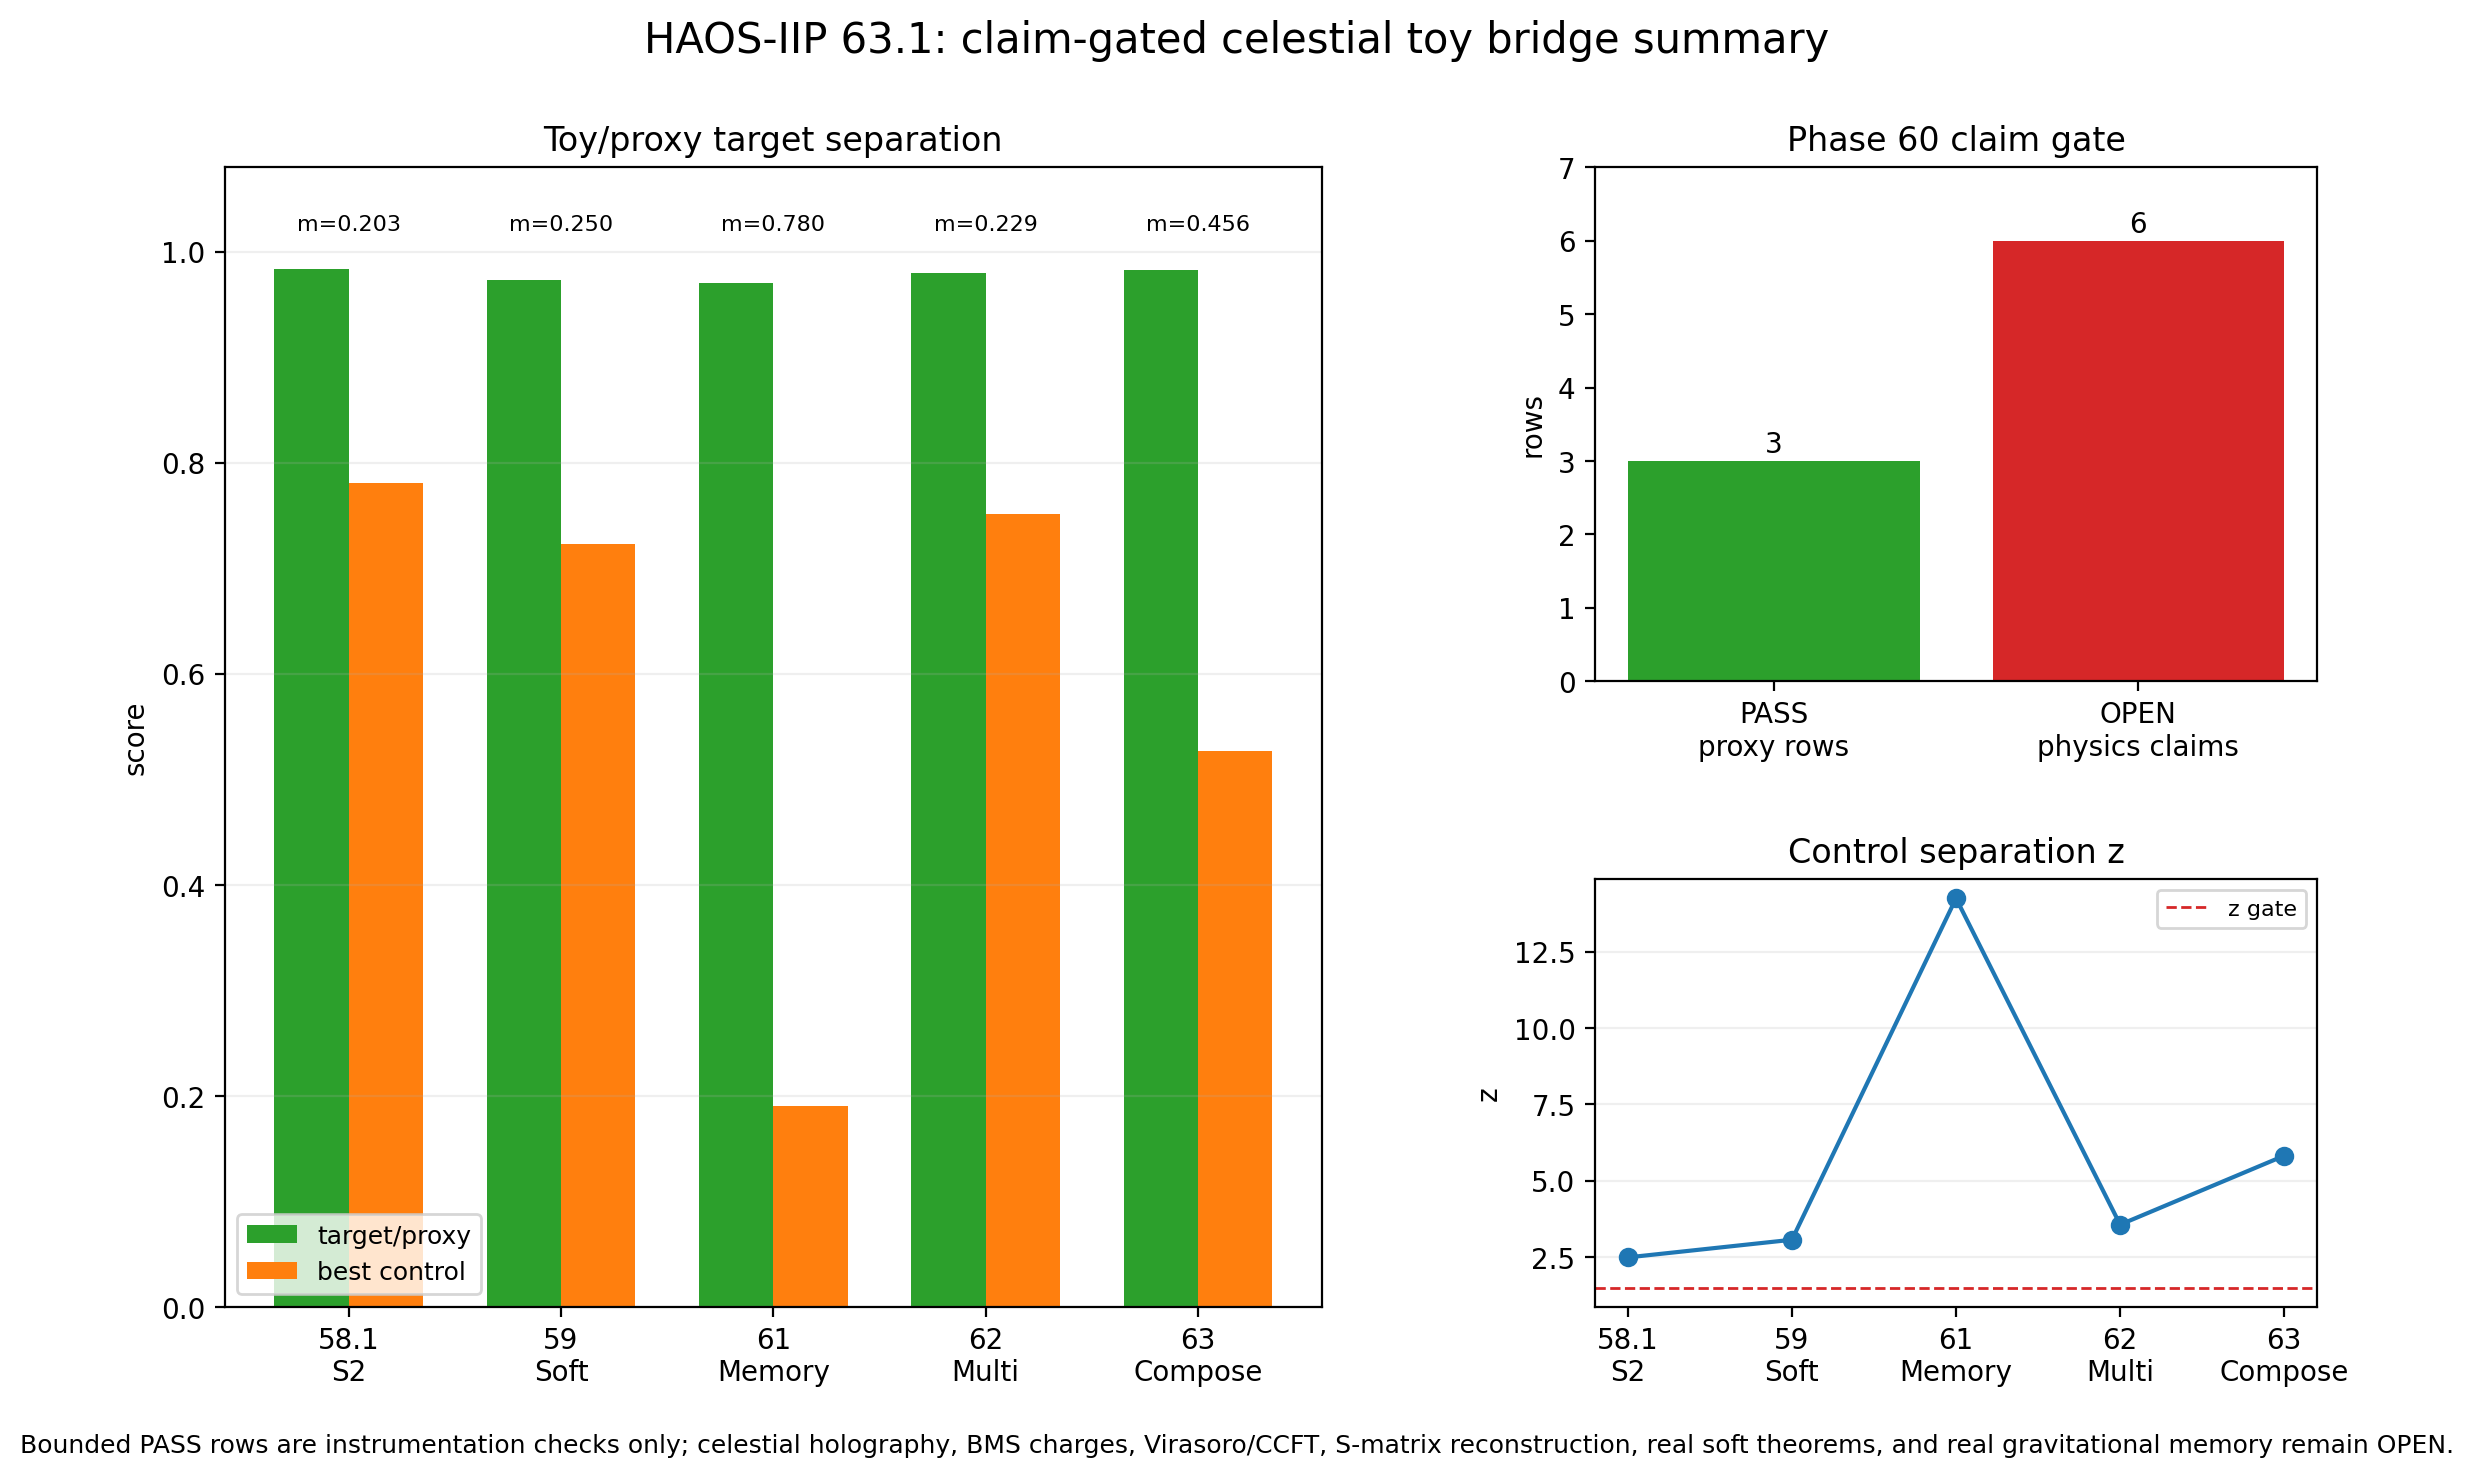
\includegraphics[width=\linewidth]{figures/phase63_1_celestial_bridge_summary.png}
\caption{Phase 63.1 visual summary. Five bounded toy/proxy probes separate their targets from best controls, while the Phase 60 claim gate keeps established physics claims open. The PASS rows are instrumentation checks only.}
\end{figure}

\section{Scope}

This paper is release \texttt{63.1} in the HAOS-IIP numbered paper sequence. It packages the work performed after the \texttt{56.5} FMO topology-contrast closure note.

The implementation lives under:
\begin{quote}
\texttt{experiments/physics\_bridge/}
\end{quote}

The relevant sidecars are:
\begin{itemize}
\item \texttt{celestial\_boundary\_audit/}
\item \texttt{spherical\_harmonic\_control\_probe/}
\item \texttt{soft\_structure\_proxy\_test/}
\item \texttt{claim\_gated\_bridge\_update/}
\item \texttt{gravitational\_memory\_toy\_probe/}
\item \texttt{multipole\_supertranslation\_probe/}
\item \texttt{supertranslation\_memory\_composition\_probe/}
\end{itemize}

No frozen HAOS-IIP core operator is modified by this release. The work is an external physics-bridge sidecar. Its purpose is to sharpen what can and cannot be said after several toy PASS results.

\section{Where the Sequence Stopped}

The previous numbered release was:
\begin{quote}
\texttt{56.5 FMO Topology Contrast and Lessons for HAOS-IIP Biology Telemetry}
\end{quote}

That paper closed the first FMO telemetry arc as a diagnostic module. The important lesson was topology sensitivity: the same spectral telemetry instrument gave a robust microtubule toy PASS, but FMO remained a productive falsifier because pathway identity and control discrimination were not strong enough on a compact, delocalized transfer graph.

The present release moves to a different question:
\begin{quote}
Can HAOS-style spectral telemetry recognize controlled boundary-geometry and soft-like toy structures without promoting those toy structures into celestial holography claims?
\end{quote}

\section{Phase 57 Boundary Audit}

Phase 57 deliberately turned the celestial-holography comparison into a boundary audit. Celestial holography starts from established asymptotic structures: BMS symmetry, soft theorems, gravitational memory, null infinity, S-matrix data, and celestial CFT correlators. HAOS-IIP does not contain those structures by default.

The audit result is:
\begin{center}
\begin{tabular}{lll}
\toprule
Phase & Status & Failure mode \\
\midrule
57 & \texttt{OPEN} & \texttt{CELESTIAL\_REQUIREMENTS\_NOT\_CLOSED} \\
\bottomrule
\end{tabular}
\end{center}

This is not a weak result. It is the necessary boundary condition for the later toy probes. The later probes can pass only as controlled instruments, not as evidence that the full celestial dictionary has been recovered.

\section{Toy and Proxy Probe Results}

\begin{center}
\begin{tabular}{llrrrr}
\toprule
Phase & Probe & Target & Best control & Margin & False positives \\
\midrule
58.1 & Spherical harmonic boundary & 0.983652 & 0.780955 & 0.202698 & 0.000000 \\
59 & Toy soft structure & 0.973247 & 0.722906 & 0.250341 & 0.000000 \\
61 & Toy displacement memory & 0.970676 & 0.190904 & 0.779772 & 0.000000 \\
62 & Multi-pole supertranslation toy & 0.980025 & 0.751041 & 0.228984 & 0.000000 \\
63 & Shift-to-memory composition toy & 0.982918 & 0.527133 & 0.455785 & 0.000000 \\
\bottomrule
\end{tabular}
\end{center}

The control-separation $z$ values are:
\begin{center}
\begin{tabular}{lr}
\toprule
Probe & Separation $z$ \\
\midrule
Spherical harmonic boundary & 2.486753 \\
Toy soft structure & 3.064268 \\
Toy displacement memory & 14.250358 \\
Multi-pole supertranslation toy & 3.559799 \\
Shift-to-memory composition toy & 5.817631 \\
\bottomrule
\end{tabular}
\end{center}

\section{Phase 58.1: Spherical Harmonic Boundary}

The spherical-harmonic probe asks a narrow boundary-geometry question: can HAOS-style spectral telemetry distinguish a known sampled $S^2$ low-mode organization from generic smooth graph spectra?

The hardened \texttt{58.1} runner adds:
\begin{itemize}
\item low-$\ell$ subspace overlap;
\item inter-band leakage checks;
\item degeneracy and band-spacing checks;
\item geodesic edge-weight signatures;
\item edgewise distance-kernel fit checks;
\item controls including coordinate permutation, weight shuffle, geodesic-bin weight shuffle, degree-preserving rewire, and ring-smooth graphs.
\end{itemize}

The result is \texttt{PASS}. The best control is \texttt{weight\_shuffle\_geodesic\_control}. The interpretation is a known-target spherical-boundary sanity check only. It is not a recovery of null infinity or celestial boundary physics.

\section{Phase 59: Toy Soft Structure}

The soft-structure proxy constructs synthetic amplitude-like rows with known pole, residue, and factorization structure. The question is whether soft-specific telemetry detects residue, pole-location, and factorization breakage better than generic smoothness.

The result is \texttt{PASS}. The target soft-specificity score is $0.973247$. The best control is the pole-location drift control, which scores $0.722906$.

This is not a real soft theorem. It is a synthetic pole/residue/factorization benchmark.

\section{Phase 60: Claim Gate}

Phase 60 is the most important discipline layer in this arc. It makes the language boundary explicit:
\begin{center}
\small
\begin{tabular}{p{0.34\linewidth}p{0.12\linewidth}p{0.42\linewidth}}
\toprule
Claim class & Status & Allowed reading \\
\midrule
Spherical harmonic boundary geometry & \texttt{PASS} & Known-target $S^2$ mode sanity check \\
Toy soft-structure proxy & \texttt{PASS} & Synthetic pole/residue/factorization sanity check \\
Claim-boundary enforcement & \texttt{PASS} & Documentation hygiene \\
Celestial holography recovery & \texttt{OPEN} & Not addressed \\
BMS charge recovery & \texttt{OPEN} & Not tested \\
Virasoro / CCFT recovery & \texttt{OPEN} & Not tested \\
S-matrix reconstruction & \texttt{OPEN} & Not tested \\
Real soft theorem recovery & \texttt{OPEN} & Not tested \\
Gravitational memory observable & \texttt{OPEN} & Not tested by Phase 60 \\
\bottomrule
\end{tabular}
\end{center}

Phases 61--63 add more toy PASS rows, but they do not close any established physics claim. They extend the toy instrumentation ladder under the same gate.

\section{Phase 61: Toy Displacement Memory}

Phase 61 creates a synthetic permanent displacement-memory pattern on a sampled $S^2$ boundary. Controls include time shuffling, transient-only bursts, coordinate permutation, wrong low-mode signatures, smooth low-mode decoys, and stochastic drift.

The result is \texttt{PASS}:
\begin{center}
\begin{tabular}{lr}
\toprule
Metric & Value \\
\midrule
target memory specificity & 0.970676 \\
recoverability & 0.999974 \\
permanence & 0.990143 \\
temporal step & 0.999998 \\
mode signature & 0.999998 \\
best control & 0.190904 \\
\bottomrule
\end{tabular}
\end{center}

This is a toy displacement-memory proxy. The real gravitational-memory observable row remains \texttt{OPEN}.

\section{Phase 62: Multi-Pole Supertranslation Toy}

Phase 62 extends the single memory target to an ordered $\ell=2,3,4$ sequence of permanent mode shifts. The first run exposed a useful leak: the \texttt{event\_order\_shuffle\_control} preserved the same final field and nearly the same multi-pole address, so final-field recovery alone was too permissive. The metric was hardened around ordered address-binding.

The final result is \texttt{PASS}:
\begin{center}
\begin{tabular}{lr}
\toprule
Metric & Value \\
\midrule
target supertranslation toy score & 0.980025 \\
final recoverability & 0.999895 \\
multipole address & 0.999904 \\
event order & 0.987852 \\
permanence & 0.995698 \\
best control & 0.751041 \\
\bottomrule
\end{tabular}
\end{center}

The best control remains \texttt{event\_order\_shuffle\_control}, as it should. It preserves much of the final field but fails the event-binding gate.

\section{Phase 63: Supertranslation--Memory Composition Toy}

Phase 63 composes the previous two ideas. A synthetic supertranslation-like shift occurs first. A later memory-like response is induced by that shift through a fixed toy response map in harmonic coefficient space.

This is stricter than testing the two fields independently. A control can preserve:
\begin{itemize}
\item the shift only;
\item the memory only;
\item the final field;
\item smoothness;
\item timing;
\item or a wrong response field,
\end{itemize}
and still fail unless the recovered memory is predicted by the recovered shift under the fixed response map.

The result is \texttt{PASS}:
\begin{center}
\begin{tabular}{lr}
\toprule
Metric & Value \\
\midrule
target composition score & 0.982918 \\
shift recoverability & 0.999969 \\
memory recoverability & 0.999800 \\
composition relation & 0.999853 \\
causal order & 0.994267 \\
address binding & 1.000000 \\
best control & 0.527133 \\
\bottomrule
\end{tabular}
\end{center}

The best control is \texttt{wrong\_shift\_right\_memory\_control}. It keeps the memory target but loses the shift-to-memory relation, which is exactly the intended failure.

\section{Interpretation}

The correct reading is:
\begin{quote}
HAOS-IIP now has a claim-gated celestial-facing toy bridge that can detect several controlled boundary and soft-like structures better than smoothness-preserving or partial-statistic controls.
\end{quote}

The equally important negative reading is:
\begin{quote}
HAOS-IIP has not recovered celestial holography, BMS charges, Virasoro/CCFT structure, a real S-matrix, real soft theorems, or real gravitational memory.
\end{quote}

Both statements must remain together. Separating them would break the point of this release.

\section{Open Limits}

\begin{itemize}
\item The spherical target is constructed and known.
\item The soft-structure proxy uses synthetic amplitude-like tables, not physical amplitudes.
\item The memory and supertranslation probes use toy fields on sampled $S^2$, not detector memory observables.
\item No BMS charge algebra is implemented.
\item No Ward identity is tested.
\item No Virasoro or celestial CFT operator algebra is recovered.
\item No S-matrix data are reconstructed.
\item No real gravitational-wave or scattering data are used.
\item The controls are strong for the toy tasks, but they are not substitutes for physical amplitudes, asymptotic charges, or observational memory data.
\end{itemize}

\section{Next Work}

The clean next steps are:
\begin{itemize}
\item update the claim-gate table with Phase 61--63 toy rows as bounded proxy rows;
\item run multi-resolution/asymptotic scaling across the spherical and memory toy families;
\item add a first explicit toy Ward-identity benchmark before using any BMS language more strongly;
\item keep all celestial-holography language under the Phase 57/60 gate until real asymptotic-symmetry or amplitude data are tested;
\item return periodically to biology and dynamics so the project does not overfit to toy celestial benchmarks.
\end{itemize}

\section{Release Artifacts}

Primary artifacts:
\begin{itemize}
\item Phase 57 celestial boundary audit runner and generated requirement table.
\item Phase 58.1 spherical harmonic control-probe runner, diagnostics, and figures.
\item Phase 59 soft-structure proxy runner, diagnostics, and figures.
\item Phase 60 claim-gated bridge table, report, and status JSON.
\item Phase 61 gravitational-memory toy runner, diagnostics, and figures.
\item Phase 62 multi-pole supertranslation toy runner, diagnostics, and figures.
\item Phase 63 supertranslation--memory composition runner, diagnostics, and figures.
\item Summary figure: \texttt{papers/figures/phase63\_1\_celestial\_bridge\_summary.png}.
\end{itemize}

The release PDF is:
\begin{quote}
63.1 Celestial Boundary Toy Probes and Claim-Gated Physics Bridge for HAOS-IIP.pdf
\end{quote}

\end{document}
